\section*{Results and Discussion}
To study the effects of multistability, non-linearities, boundaries and growth, we use a simple model which consists of a 2-node Turing topology system with non-linear Hill terms.
The activator A activates itself and I, while the inhibitor I inhibits the activator A.
However, instead of using the linear terms used in the original Turing system~\parencite{Turing1952}, we use Hill terms which represent genetic regulations.

\begin{subequations}
    \begin{equation}
        \pdv{[A]}{t}=b_{A}+V_{A} \cdot\frac{1}{1+\left(\frac{K{A}}{[A]}\right)^{n_{A}}}\cdot\frac{1}{1+\left(\frac{[I]}{K_{I}}\right)^{n_{I}}}-\mu_{A}\cdot[A] + D_{A}\nabla^2 [A]
    \end{equation}

    \begin{equation}
        \pdv{[I]}{t}=b_{I}+V_{I} \cdot\frac{1}{1+\left(\frac{K{A}}{[A]}\right)^{n_{A}}}-\mu_{I}\cdot[I] +
        D_{I}\nabla^2 [I]
    \end{equation}

    \label{eq:turinghill}
\end{subequations}
\subsection*{Multistability}
In this section, we demonstrate how linear stability analysis is not sufficient or necessary to predict Turing patterns (TPs) in multi-stable systems.
In particular, we study in detail the dynamical behaviour of multi-stable systems during pattern formation, which will lead to the creation or breaking of the pattern.
The motivation behind this arises from the high degree of multistability exhibited by biological systems, where cell-fate decisions have to be taken within this landscape ~\parencite{huang2000shape, moris2016transition}.
Multistability is especially common in systems with non-linearities and feedback loops, as the ones in biology or in our models~\parencite{pham2020complexity, leite2009multistability}.

Using the two-node non-linear Turing topology (Eq.~\ref{eq:turinghill}), multi-stable solutions were found and studied to understand how the patterning dynamics get affected when multiple steady-state solutions are found.
First, LSA is carried out on particular parameter sets to find multiple steady states with different stability nature (e.g.~stable, unstable, Turing I, Turing I-Hopf).
Then numerical simulations are computed where the initial condition is a random uniform distribution around a particular steady state.
Different pattern outcomes result depending on where in the phase diagram the initial condition is.
Following the classical hypothesis used in the Turing robustness literature, we would expect stable and unstable systems to not produce patterns and Turing to produce patterns.
Here, we present various examples of how this hypothesis can break under multistability conditions.

Fig.~\ref{fig:multistability1} shows a case where diffusion-driven instability conditions are not required for Turing pattern formation.
The unstable state, having a dispersion relation with a peak below zero (Fig.~\ref{fig:multistability1}C), managed to get into a Turing pattern regime as it is attracted by the neighbouring Turing steady state.
It therefore produces a stationary pattern (Fig.~\ref{fig:multistability1}B), even though its dispersion relation does not predict so.
This trajectory is depicted in the phase diagram (Fig.~\ref{fig:multistability1}A) which shows the steady states along with the vector field to understand the potential trajectories of the system.
The phase diagram does not fully capture the dynamics as it describes the system without diffusion, while the dispersion relation and the numerical solution do consider diffusion.

\begin{figure}[H]
    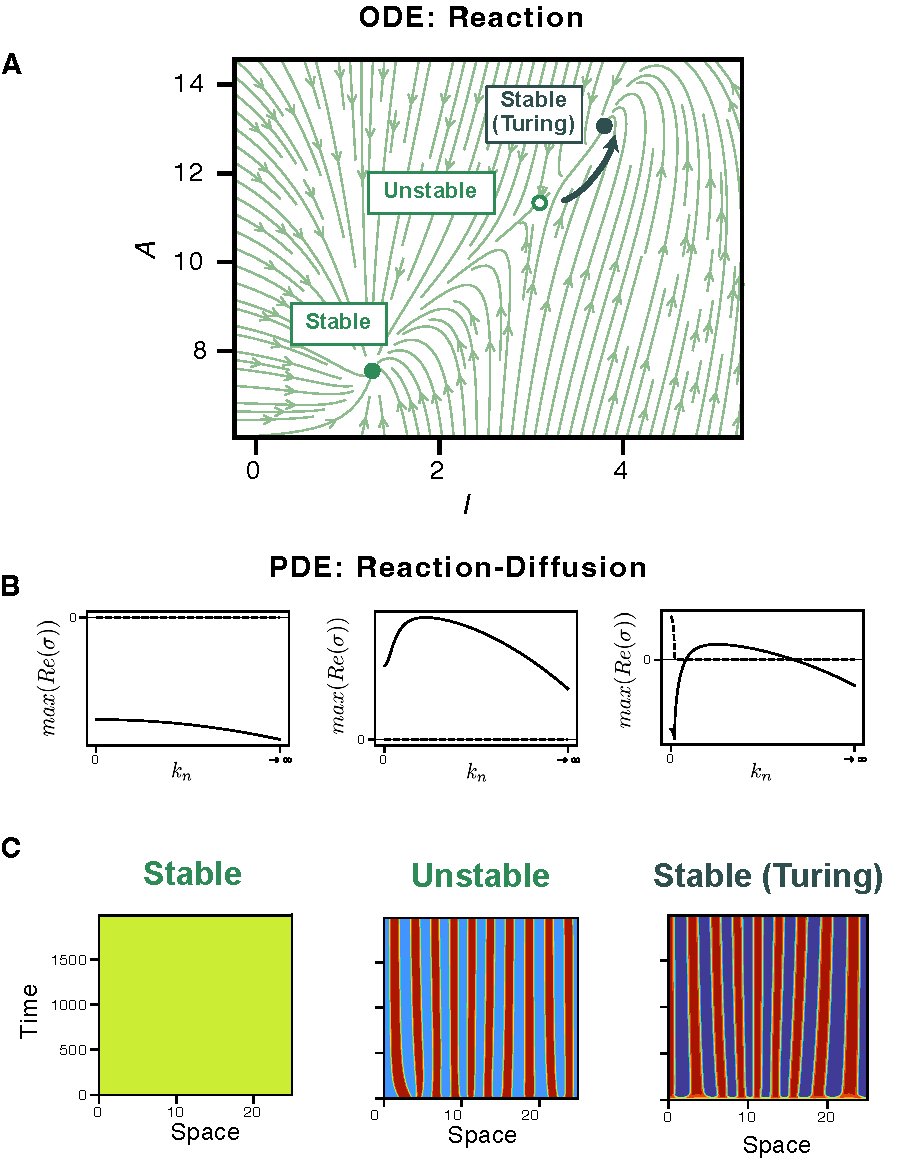
\includegraphics[width=1\textwidth]{figures/multistability1}

    \caption{\textbf{Stationary Patterns in multistability.} \textbf{(A)} Phase diagram without diffusion illustrating three distinct steady states where the derivative is zero: stable, unstable, and stable (Turing). These steady states are represented within a parameter space defined by two axes: concentrations of A and I. The vector field, indicated by light green arrows, shows the direction of the derivatives of the system at various points in the parameter space. A hand-drawn trajectory is also shown (dark green arrow), demonstrating how the unstable state may evolve into the Turing state. \textbf{(B)} Dispersion relation showing each type of state. \textbf{(C)} Numerical solutions of the three steady states with diffusion, where the unstable state unexpectedly produces a Turing-like stationary pattern. }
    \label{fig:multistability1} % A label for referencing this figure later in the document
\end{figure}



Then, we present a case where LSA incorrectly predicts stationary pattern formation.
Fig.~\ref{fig:multistability2} shows an ephemeral or transient pattern that occurs in the unstable and Turing regimes.
The TP initially develops in the vicinity of the Turing steady state.
As the spatial heterogeneity is amplified and settles, it gets attracted by the stable steady state leading to the disruption of the pattern.
This type of transient pattern behaviour has also been recently reported in~\cite{Krause2023}.

\begin{figure}[H]
        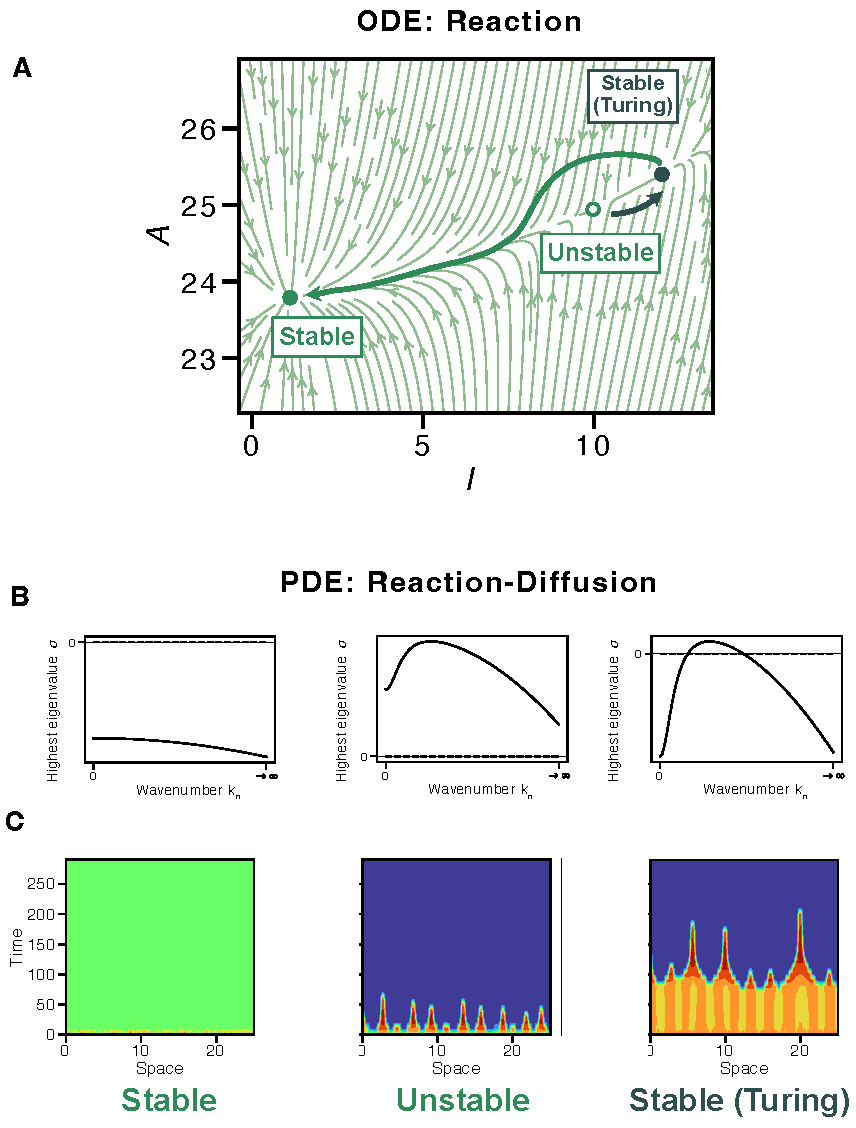
\includegraphics[width=1\textwidth]{figures/multistability2} % The name of your image file; assumes it is in the same directory as your .tex file
    \caption{\textbf{Ephemeral patterns in multistability.} \textbf{(A)} Phase diagram without diffusion illustrating three distinct steady states where the derivative is zero. The hand-drawn trajectory (dark green arrow) shows an unstable state evolving into a stable (Turing), and a stable (Turing) evolving into a stable. \textbf{(B)} Dispersion relation showing each type of state. \textbf{(C)} Numerical solutions of three steady states with diffusion. Unstable and Turing produce temporary periodic stationary patterns, that then disappear and become spatially homogeneous solutions.}
    \label{fig:multistability2} % A label for referencing this figure later in the document
\end{figure}

Other interesting examples can be found, for example, where an unstable state is surrounded by two Turing states, this unstable state will robustly lead to a Turing pattern (Fig.~\ref{sup_fig4}A).
Additionally, in some cases, the unstable system settles into Turing, but the Turing system gets pulled by the stable attractor (Fig.~\ref{sup_fig4}B). Additionally, some systems even exhibit three solutions which are homogeneous in time and space (Fig.~\ref{sup_fig4}C).
In this case, it would be worth investigating earlier time points with more resolution, as a pattern might appear then.
Interesting interactions similarly occur with multistability involving Turing I-Hopf solutions which will be mentioned in the following sections (Fig.~\ref{sup_fig4}D).



\subsection{Analytical to numerical: Other types of dispersion relations, and other types of patterns} \label{nogrowth}
Multi-stable systems are not the only case where the classical Turing instability theory fails to predict pattern formation.
Other types of dispersion relations beyond classical Turing instabilities can produce stationary patterns and non-stationary regular patterns that might be of interest in developmental biology.

High-throughput studies like~\cite{Scholes2019, Zheng2016, Marcon} only consider Turing I as patterning and the rest is discarded.
Here we explore beyond Turing I and stationary patterns to give a more complete view of the relationship between linear stability and spatio-temporal patterns.
By classifying dispersion relation types and pattern types, we document what type of dispersion relations in mono-stable systems can be linked to what type of patterns, to gain insights into predicting pattern formation from linear stability analysis.
All types of dispersion relations in our parameter space were classified into 5 types:
\begin{itemize}
    \item Stable dispersion relations (Fig~\ref{fig:dispersions}A) have all eigenvalues $\sigma$ below zero for any wavenumber $k_{n}$.
    \item Unstable dispersion relations (Fig~\ref{fig:dispersions}C) have a positive eigenvalue at $k_{0}=0$ which eventually drops below zero as diffusion is introduced (i.e. $k_{n}>0$).
    \item Hopf-type dispersion relations, as with any unstable dispersion relation, shows an instability without diffusion ($\sigma>0$ for $k_{0}=0$) which eventually drops below zero for positive wavenumbers.
    However, in the case of the Hopf-type dispersion relation, when the eigenvalues cross the zero line, there is a pair of complex conjugate eigenvalues (Fig~\ref{fig:dispersions}D).
    A Hopf-like dispersion relation is different to a Hopf bifurcation: a bifurcation displays a shift in stability as a model parameter changes, while the Hopf-like dispersion is a change in stability as a function of the wavenumber $k_{n}$.
%In this case, the bifurcation parameter would be $k$, making the system go from unstable to stable by changing this parameter.
    \item Turing I dispersion relations, as previously mentioned, are stable without diffusion, have an instability for a positive wavenumber, and finally become stable again for very large wavenumbers (Fig~\ref{fig:dispersions}B).
    \item Turing I-Hopf dispersion relations, are a combination of Turing I and Hopf-type dispersion relations.
    As the Hopf-type dispersion, they are unstable without diffusion.
    Then, as $k_{n}$ is increased, the system becomes stable with a pair of complex conjugates as the eigenvalues cross the zero line.
    Finally, a Turing I-type behaviour arises getting a peak above zero and decaying again for large wavenumbers (Fig~\ref{fig:dispersions}E).
\end{itemize}
Other types of dispersion relation exist which are not displayed here such as Turing II, where the eigenvalues do not become stable again for very large wavenumbers.
Therefore, this system displays an instability at very large wavenumbers which results in infinitesimally small wavelength patterns.
These are considered to produce homogeneous solutions, except in the case of space discretization where they can produce small wavelength patterns~\parencite{Wang2022}.
However, Turing II solutions are not possible in systems such as this one where all nodes are diffusing.
This is because for $k_n \rightarrow \inf$, all eigenvalues $\sigma$ must be negative (see Eq.~\ref{jacobian_diffusion}).

As with the classification of the dispersion relations, we classify the patterns produced numerically into homogeneous, temporal oscillator, non-stationary pattern and stationary pattern.
By classifying both LSA and numerical outputs, we can generate a new confusion matrix with information about other types of dispersion relations and other types of spatio-temporal patterns (Fig~\ref{fig:dispersions}F).

This confusion matrix shows how not only systems with a Turing I dispersion relations can generate a stationary spatial pattern. Unstable, Hopf and Turing I Hopf can produce such results too. Additionally, interesting behaviours can arise such as temporal oscillators and non-stationary patterns.

\begin{figure}[H]
    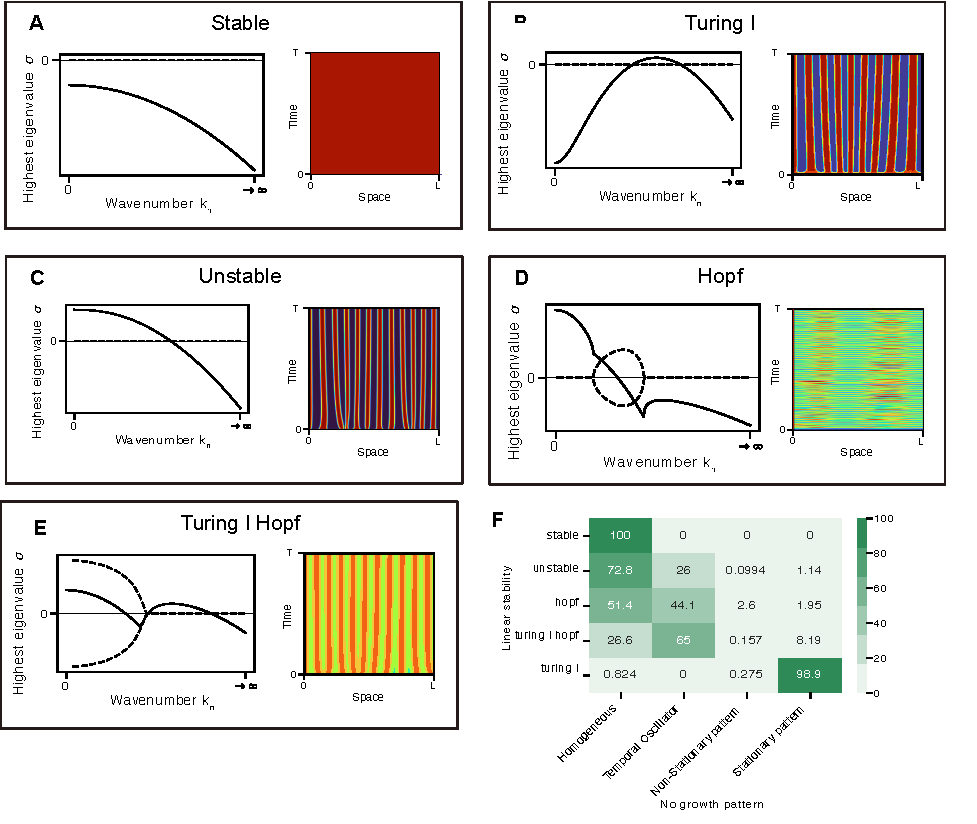
\includegraphics[width=1\textwidth]{figures/dispersion} % The name of your image file; assumes it is in the same directory as your .tex file
    \caption{\textbf{Relationship between dispersion relation and numerical solutions} \textbf{(A-E)} Examples of a dispersion relation (left) and a resulting numerical solution (right) for Stable, Turing I, Unstable, Hopf, Turing I Hopf. \textbf{(F)} Confusion matrix linking LSA output (rows) and numerical pattern outcome (columns). Numbers show the percentage of solutions across the LSA output rows.}
    \label{fig:dispersions} % A label for referencing this figure later in the document
\end{figure}

\textbf{Confusion matrix linking LSA output (rows) and numerical pattern outcome (columns).} Numbers show the percentage of solutions across the LSA output rows.

\section{Introducing biological features: Absorbing boundaries and growth}
As shown above, both multistability effects and numerical solutions can break the hypothesis that only classical Turing I systems can produce stationary periodic patterns.

Here, we look deeper into how other aspects linking the theory closer to the biological reality can also break this hypothesis.
In particular, we will look at how adding an absorbing boundary condition and growth to a reaction-diffusion system might induce or break patterning.
This particular direction was inspired by experiments described in the next sections where growing bacterial colonies in agar are used as a platform to engineer Turing patterns using synthetic gene circuits.

The parameter space was explored using simulations and classifying these simulations with no-flux and no-growth conditions, absorbing boundary conditions and growth.
Again, all these parameter sets have only a single steady state to ensure patterning effects are due to boundaries and growth and not due to multistability.

\begin{figure}[H]
    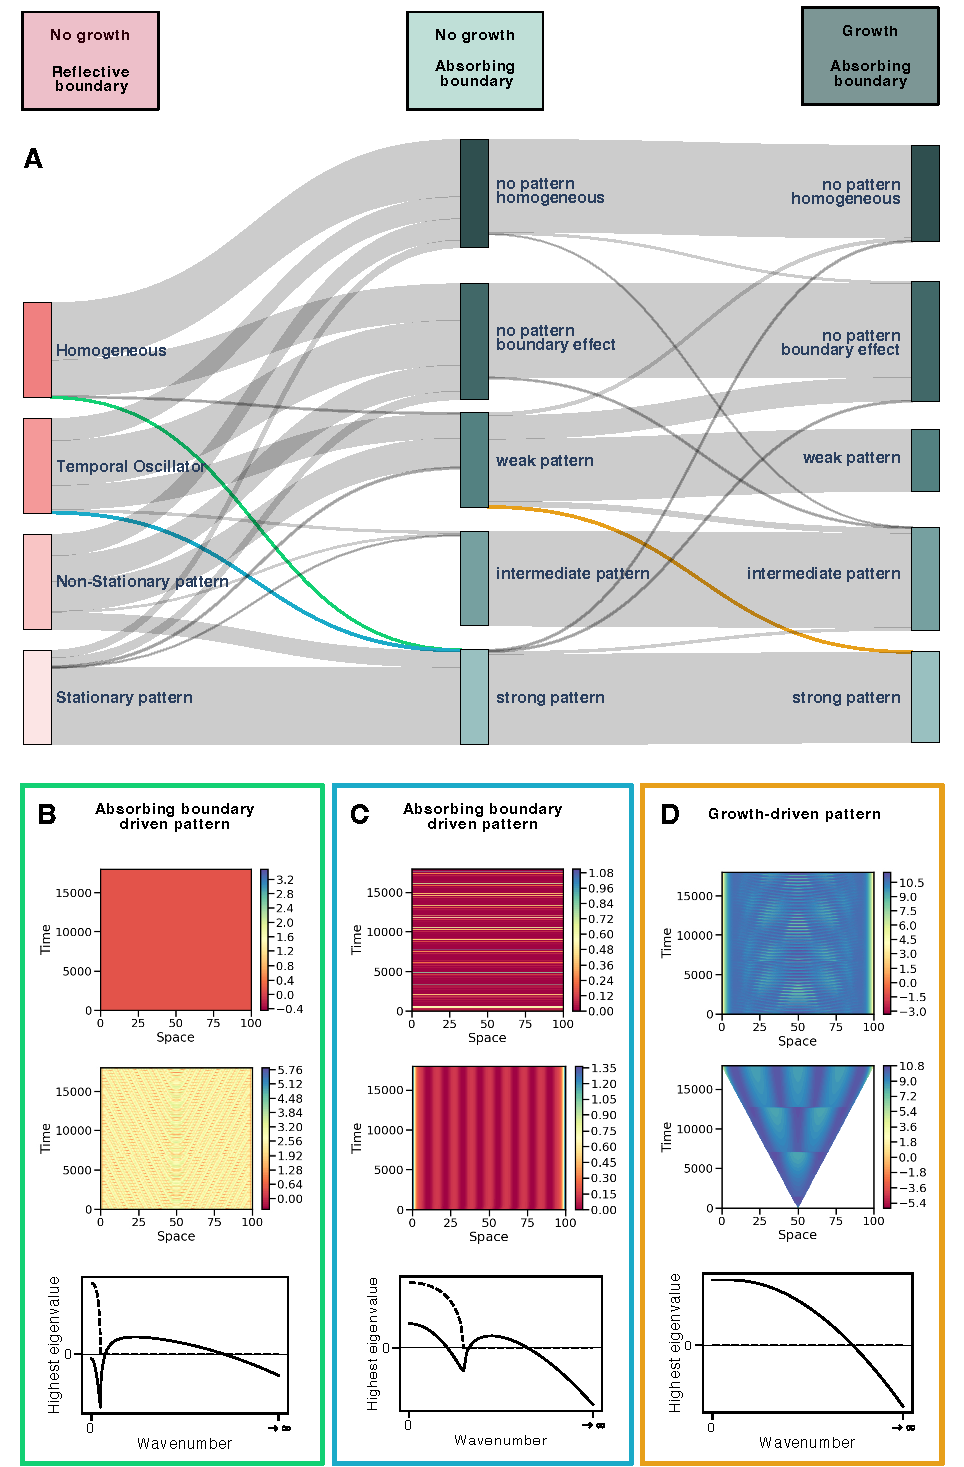
\includegraphics[width=1\textwidth]{figures/boundaries_growth} % The name of your image file; assumes it is in the same directory as your .tex file
    \caption{a}
    \label{fig:boundariesgrowth} % A label for referencing this figure later in the document
\end{figure}

When absorbing boundaries are added, periodic patterns might get created, disrupted or remain the same. The Sankey diagram in Fig~\ref{fig:boundariesgrowth}A shows how this system can transition when absorbing boundaries and growth are introduced.
As previously explained, the no-growth classification could not be used for absorbing boundary conditions as these prevent the pattern from being completely homogeneous or stationary. %TODO ref classification. %TODO add letter to image
Therefore, two types of classifications have to be compared for each type of boundary.
Although the classification outputs cannot be directly compared, this confusion matrix is useful to identify interesting cases:
If absorbing boundary conditions had no effect, we would expect homogeneous and temporal oscillator categories in the y-axis to become no pattern, homogeneous or boundary effect.
Additionally, we would expect stationary patterns to become strong patterns.
This is commonly the case as seen by the thicker lines in, which shows boundaries do not often affect the pattern.
However, some exceptions are present which are further studied in Fig~\ref{fig:boundariesgrowth}B.
